\documentclass[]{report}
\usepackage{amsmath}
\usepackage{amssymb}
\usepackage[english]{babel}
\usepackage[utf8]{inputenc}
\usepackage[T1]{fontenc}
\usepackage{euler}

\usepackage[inner=0cm,outer=0cm,top=0.3cm,bottom=0cm,paperwidth=14cm,paperheight=8cm]{geometry}

\usepackage{tikz,pgfplots}
\usetikzlibrary{positioning}
\usetikzlibrary{decorations.pathmorphing}

\begin{document}
\centering
	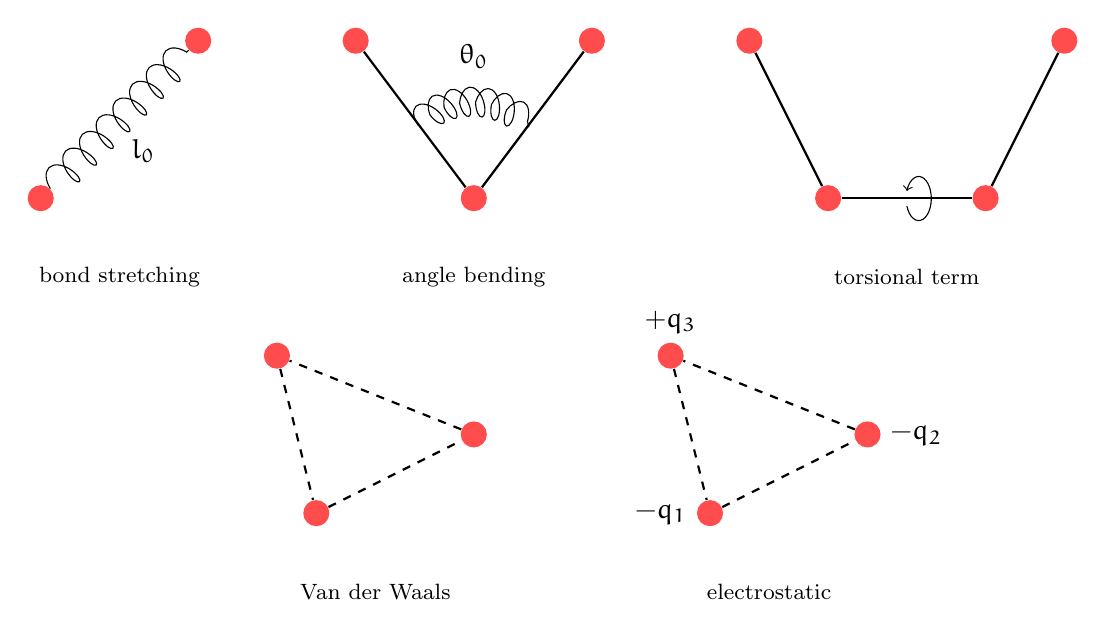
\begin{tikzpicture}
		%\draw[thin, gray!25] (0,0) grid (15,8);
		\node[fill=red!70, circle, radius=0.15] (1) at (0,6) {};
		\node[fill=red!70, circle, radius=0.15] (2) at (2,8) {};
		\draw[decorate, decoration={coil,segment length=3mm,amplitude=2mm}] (1) -- (2);
		\node[] at (1.3,6.6) {$l_0$};
		\node[] at (1,5) {\footnotesize bond stretching};
		\node[fill=red!70, circle, radius=0.15] (3) at (4,8) {};
		\node[fill=red!70, circle, radius=0.15] (4) at (5.5,6) {};
		\node[fill=red!70, circle, radius=0.15] (5) at (7,8) {};
		\draw[thick,-] (3) -- (4) node[midway] (mid1) {};
		\draw[thick,-] (4) -- (5) node[midway] (mid2) {};
		\draw[-,decorate, decoration={coil,segment length=2mm,amplitude=2mm}] (4.8,6.91924) to[out=45,in=135] (6.2,6.9);
		\node[] at (5.5,7.8) {$\theta_0$};
		\node[] at (5.5,5) {\footnotesize angle bending};
		\node[fill=red!70, circle, radius=0.15] (6) at (9, 8) {};
		\node[fill=red!70, circle, radius=0.15] (7) at (10, 6) {};
		\node[fill=red!70, circle, radius=0.15] (8) at (12, 6) {};
		\node[fill=red!70, circle, radius=0.15] (9) at (13, 8) {};
		\draw[thick,-] (6) -- (7);
		\draw[thick,-] (7) -- (8);
		\draw[thick,-] (8) -- (9);
		\draw[->] (11,5.9) arc [start angle=-160, end angle=160, x radius=0.16cm, y radius=0.28cm];
		\node[] at (11,5) {\footnotesize torsional term};
		\node[fill=red!70, circle, radius=0.15] (10) at (3,4) {};
		\node[fill=red!70, circle, radius=0.15] (11) at (3.5, 2) {};
		\node[fill=red!70, circle, radius=0.15] (12) at (5.5, 3) {};
		\draw[thick,dashed] (10) -- (11);
		\draw[thick,dashed] (11) -- (12);
		\draw[thick,dashed] (12) -- (10);
		\node[] at (4.25,1) {\footnotesize Van der Waals};
		\node[fill=red!70, circle, radius=0.15, label=above:$+q_3$] (13) at (8,4) {};
		\node[fill=red!70, circle, radius=0.15, label=left:$-q_1$] (14) at (8.5, 2) {};
		\node[fill=red!70, circle, radius=0.15, label=right:$-q_2$] (15) at (10.5, 3) {};
		\draw[thick,dashed] (13) -- (14);
		\draw[thick,dashed] (14) -- (15);
		\draw[thick,dashed] (15) -- (13);
		\node[] at (9.25,1) {\footnotesize electrostatic};
	\end{tikzpicture}
\end{document}
	